\section{Тематическое моделирование}

Тематическая модель (англ. \textit{topic model}) — модель коллекции текстовых документов, которая определяет, к каким темам относится каждый документ коллекции. Алгоритм построения тематической модели получает на входе коллекцию текстовых документов. На выходе для каждого документа выдаётся числовой вектор, составленный из оценок степени принадлежности данного документа каждой из тем. Размерность этого вектора, равная числу тем, может либо задаваться на входе, либо определяться моделью автоматически.

Тематическое моделирование (англ. \textit{topic modeling}) — построение тематической модели.

Задача построения тематической модели звучит следующим образом. Задана коллекция текстовых документов $D$. Каждый документ $d$ из коллекции $D$ представляет собой последовательность слов $W_d=(w_1,\ldots,w_{n_d})$ из словаря $W$, где $n_d$ — длина документа $d$. Предполагается, что каждый документ может относиться к одной или нескольким темам. Темы отличаются друг от друга различной частотой употребления слов. Требуется найти эти темы, то есть определить
\begin{itemize}
\item число тем;
\item распределения частот слов, характерное для каждой темы;
\item тематику каждого документа — в какой степени он относится к каждой из тем.
\end{itemize}

Данная задача может рассматриваться как задача одновременной кластеризации документов и слов по одному и тому же множеству кластеров, называемых темами. Строится, так называемая, мягкая кластеризация, то есть один документ может принадлежать нескольким темам в различной степени.

Для тематического моделирования в качестве модели в данной работе используется латентное размещение Дирихле (англ. \textit{latent Dirichlet allocation, LDA}) \cite{bib4}.

Для оценки качества данной модели используется перплексия (англ. \textit{perplexity}) --- оценка того, насколько хорошо вероятностная модель предсказывает выборку. Низкая перплексия указывает на то, что распределение вероятностей хорошо предсказывает выборку. 

В зависимости от параметра модели, отвечающего за количество тем у распределения текстов, получилась следующая зависимость значения перплексии от количества тем:

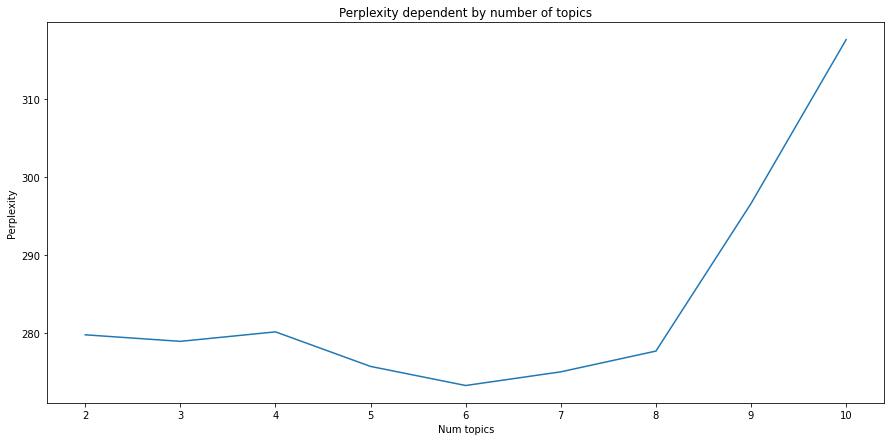
\includegraphics[scale=0.5]{pics/perplexity.png}

Ниже приведены примеры слов, принадлежащие каждой из 6 (с оптимальным значением перплексии) тем:

\begin{tabular}{ | l | l | l | }
\hline
Номер темы & Слова \\ \hline
1 & obama, state, president, government, american, \\ & israel,  policy, country \\ \hline
2 & woman, say, work, health, year, senate, group, \\ & government,  support, company \\ \hline
3 & call, get, work, see, want, know, good, also, think, tomorrow \\ \hline
4 & secretary, office, state, meet, room, department,  \\ &  arrive, route, depart, private \\ \hline 
5 & state, information, benghazi, department, doc, case, subject, \\ & iran, agreement, house \\ \hline
6 & cheryl, gov, fyi, sullivan, state, friday, sunday, branch,  \\ & wednesday, april, january \\ \hline 

\end{tabular}

\newpage

Распределение слов по темам:

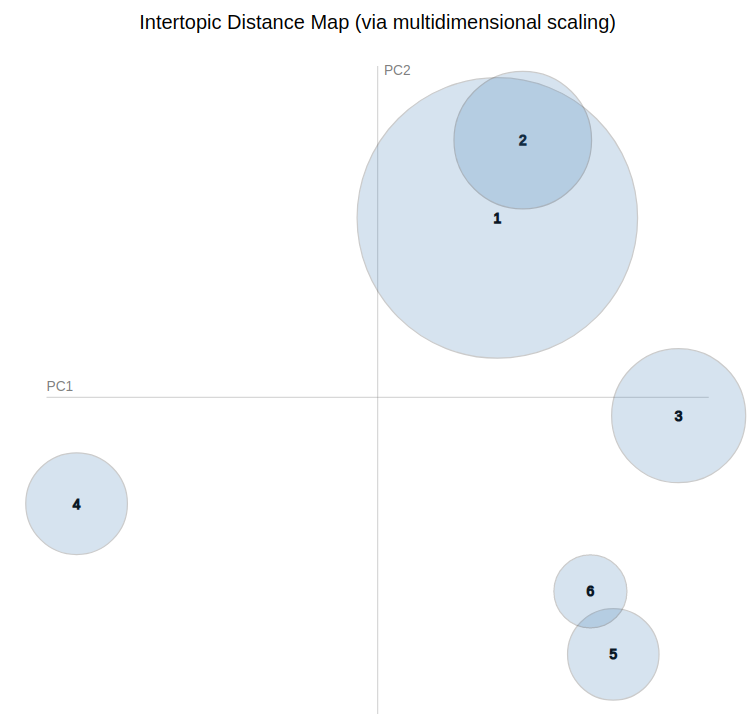
\includegraphics[scale=0.5]{pics/words_map.png}

